\chapter{Implementación}
\label{chap:implementacion}

A lo largo de este capítulo, se expondrán las decisiones de implementación más relevantes tomadas durante el desarrollo del proyecto.

\section{\textit{Backend}}

Para analizar la implementación del \textit{backend}, se tomará como referencia el diagrama de clases de la Figura \ref{fig:implementacion_clases_backend} y se profundizará
en las clases más importantes que lo componen. Asimismo, se estudirá y se justificará cuales han sido los \textit{endpoints} expuestos por el servidor,
representados en la Figura \ref{fig:implementacion_endpoints}.

\subsection{\textit{Endpoints}}

Dado que el \textit{backend} seguirá una arquitectura REST, se explicarán a continuación los \textit{endpoints} que se han implementado para el servidor, así como los parámetros
que recibe cada uno. Como se puede observar en la Figura \ref{fig:implementacion_endpoints}, el servidor expone un total de cuatro \textit{endpoints}:

\begin{itemize}
	\item \textbf{/predict}: Como indica la historia de usuario con identificador \textit{1} de la Sección \ref{sec:analisis_requisitos_funcionales}, el usuario
		debe poder subir su propio dataset de textos para su perfilado. Para ello, se ha implementado este \textit{endpoint} que recibe como parámetros de la URL el
		nombre del algoritmo de perfilado a utilizar junto al \textit{dataset} utilizado para entrenar el modelo. Además, ya que el método de la petición es POST,
		será en el cuerpo donde se envíe
		el archivo con los textos a perfilar. En caso de que el archivo no sea correcto, que el algoritmo no exista o que el \textit{dataset} de entrenamiento
		no sea válido, se devolverá un error HTTP 400 (\textit{Bad Request}). En caso contrario, se devolverá un identificador correspondiente a la tarea de perfilado
		que se ha creado de forma asíncrona, generado dinámicamente con la librería uuid \cite{uuidpython} de Python (según el estándar RFC 4122 \cite{rfc4122}) y que coincide
		con el identificador del documento almacenado en la base de datos. 
		El hecho de no esperar a que el perfilado se complete 
		para devolver una respuesta al usuario evita tener problemas con el tiempo de espera de la petición o \textit{timeout} del \textit{socket} TCP, 
		permitiendo así procesar grandes volúmenes de datos y cumplir con el requisito de escalabilidad establecido en la Sección \ref{sec:analisis_requisitos_no_funcionales}.

	\item \textbf{/train}: Además, ya que el usuario debe poder reentrenar los modelos con los algoritmos disponibles, se ha implementado este \textit{endpoint} de tipo GET.
		En este caso, se recibe como parámetros de la URL el nombre del algoritmo de perfilado a utilizar junto al \textit{dataset} de entrenamiento. De la misma forma,
		se validarán los parámetros y, en caso de que sean correctos, se iniciará una tarea asíncrona en el \textit{backend}.

	\item \textbf{/performance}: Puesto que otra de las historias de usuario nos indica que es necesario conocer el rendimiento que tiene los algoritmos,
		el \textit{backend} expondrá otro \textit{endpoint} de tipo GET que recibe los mismos parámetros que el anterior. La diferencia es que, en este caso,
		se devolverá un JSON con los valores de rendimiento del algoritmo en lugar de iniciar una tarea asíncrona.
	
	\item \textbf{/profilings/\{id\}}: Para poder obtener los resultados del perfilado creado de forma asíncrona, este \textit{endpoint} de tipo GET
		permite recuperarlos de la base da datos haciendo uso del identificador devuelto por la tarea de predicción. En caso de que la tarea
		no exista, se devolverá un error HTTP 404 (\textit{Not Found}). La respuesta devuelta será un JSON con la estructura mostrada en la Figura \ref{fig:profiling_json}.

		\begin{figure}[H]
			\begin{lstlisting}[language=json]
{
	"status": "SUCCESS",
	"algorithm": "martinc",
	"time": 4291,
	"output": [
		{
			"id": "29502",
			"result": {
				"gender": "male",
				"fame": "star",
				"occupation": "sports",
				"age": "35-49"
			}
		},
		{
			"id": "38991",
			"result": {
				"gender": "female",
				"fame": "rising",
				"occupation": "performer",
				"age": "50-XX"
			}
		},
	]
}\end{lstlisting}
			\caption{Estructura del JSON devuelto por el \textit{endpoint} /profilings/\{id\}}
			\label{fig:profiling_json}
		\end{figure}
\end{itemize}

Destacar que en todos los casos, tanto el algoritmo de Grivas et al. \cite{grivas2015author} como el de Martinc et al. \cite{martinc2019hot}, tienen asociado un \textit{dataset} de entrenamiento por defecto (que coincide
con el utilizado por los autores originales en su publicación), el cual se utilizará en caso de no especificar ninguno en la URL.

\begin{figure}[H]
	\centering
	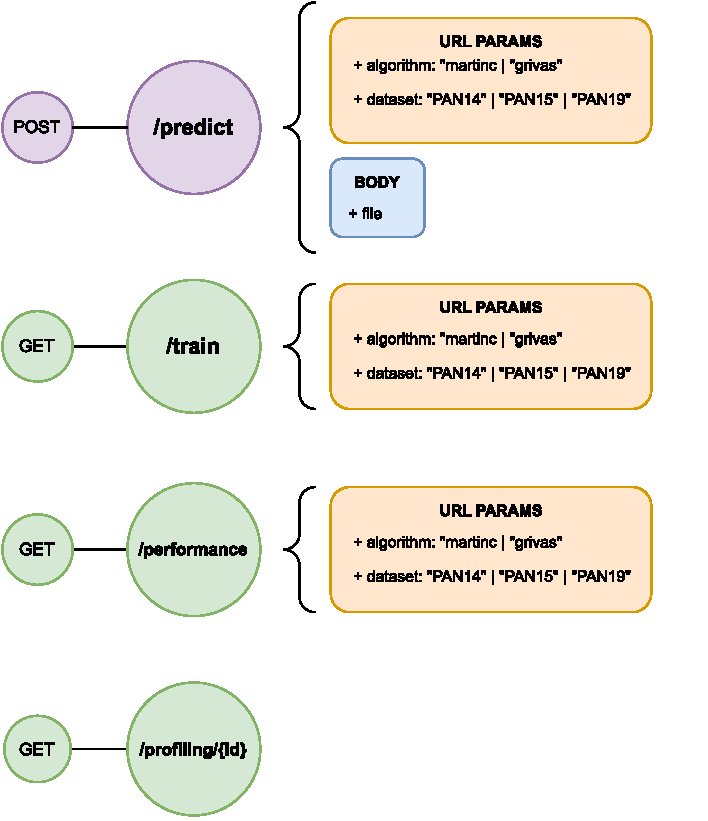
\includegraphics[width=0.5\textwidth]{diagramas/endpoints.pdf}
	\caption{Diagrama de \textit{endpoints} del \textit{backend}}
	\label{fig:implementacion_endpoints}
\end{figure}

\subsection{Clases}

\bigskip
Como se explicó en la Sección \ref{sec:herramientas_backend}, la estructura del \textit{backend} sigue los principios
del patrón de diseño DDD \cite{ddd}, en el que se distinguen tres capas: la capa de aplicación, la capa de dominio
y la capa de infrastructura.

\bigskip
Nuestro punto de entrada al sistema, es decir, el componente que forma parte de la \textbf{capa de aplicación}, es la clase
\textit{Controller}, el cual se encarga de realizar las siguientes tareas:

\begin{itemize}
	\item Exponer los \textit{endpoints} y recibir los parámetros de entrada, ya sea a través de la URL o del cuerpo de la petición
	haciendo uso de FastAPI \cite{fastapi}.
	\item Validar dichos parámetros y devolver los errores HTTP correspondientes en caso de que no sean correctos.
	\item Parsear los parámetros de entrada a los tipos de datos que se necesiten.
	\item Realizar la llamada al servicio de la capa de dominio y devolver el valor de retorno encapsulado en una respuesta HTTP.
\end{itemize}

\bigskip
En la \textbf{capa de dominio}, una vez los datos han sido validados y parseados, el \textit{ProfilingService} es el encargado de orquestar
las diferentes llamadas y delegar la lógica de negocio a las distintas entidades.

\bigskip
La más importante de ellas es la clase \textit{ProfilingAlgorithm},
una clase abstracta que define la interfaz que deben implementar todos los algoritmos de perfilado incluyendo las tres funciones principales:
\textit{predict()}, \textit{train()} y \textit{get\_performance()}. En este sentido, es importante mencionar que los algoritmos elegidos no estaban implementados
pensando en formar parte de una aplicación más grande, por lo que fue necesario realizar una adaptación manual para cumplir con la interfaz de
la clase heredada, lo que implicó comprender a muy bajo nivel como estaban implementados dichos algoritmos. Esta adaptación del código fue, en el caso del algoritmo de Grivas et al. \cite{grivas2015author}, 
bastante compleja, ya que conllevó sustituír librerías obsoletas, reimplementar funciones y actualizar la sintaxis a la nueva versión de Python.

\bigskip
Otra entidad importante de la capa de dominio es la clase \textit{PredictDataset}, que representa el \textit{dataset} que proporciona el usuario
para realizar la predicción. Dado que los algoritmos de perfilado requieren que el \textit{dataset} tenga un formato específico (en este caso
ambos solo procesan NDJSON), es necesario implementar conversores que transformen el archivo de entrada a dicho formato por lo que
fue necesario crear las clases \textit{CsvToNdjsonConverter} y \textit{NdjsonToCsvConverter}.

\bigskip
También existe una clase llamada \textit{TrainDataset}, que representa
el \textit{dataset} que se utiliza para entrenar y validar el modelo. Esta clase abstracta contiene la locacalización de los elementos
del conjunto de entrenamiento y test, así como también un nombre que la identifica. Esto nos permite la incorporación de nuevos \textit{datasets} creando simplemente
una nueva clase que herede de \textit{TrainDataset}, posibilitando la generación de modelos haciendo uso de diferentes conjuntos de entrenamiento de forma sencilla y automática. 

\bigskip
Finalmente, en la capa de dominio, se encuentra la clase abstracta \textit{ProfilingRepository}, la cual define la interfaz que deben implementar
los repositorios de tecnologías de bases de datos concretas, ya sean relacionales, no relacionales o de otro tipo.

\bigskip
Ya en la \textbf{capa de infraestructura}, es decir, donde se almacenan todos los componentes externos con los que interactúa el dominio, se encuentran las clases que implementan
la interfaz definida por el \textit{ProfilingRepository}. En nuestro caso, ya que se decidió optar por MongoDB como base de datos, solo existe
la clase \textit{MongoProfilingRepository}, la cual se encarga de realizar las operaciones CRUD (del inglés \textit{Create, Read, Update, Delete}) sobre la base de datos, así
como de establecer y mantener la conexión con la misma.

\bigskip
\begin{figure}[H]
	\centering
	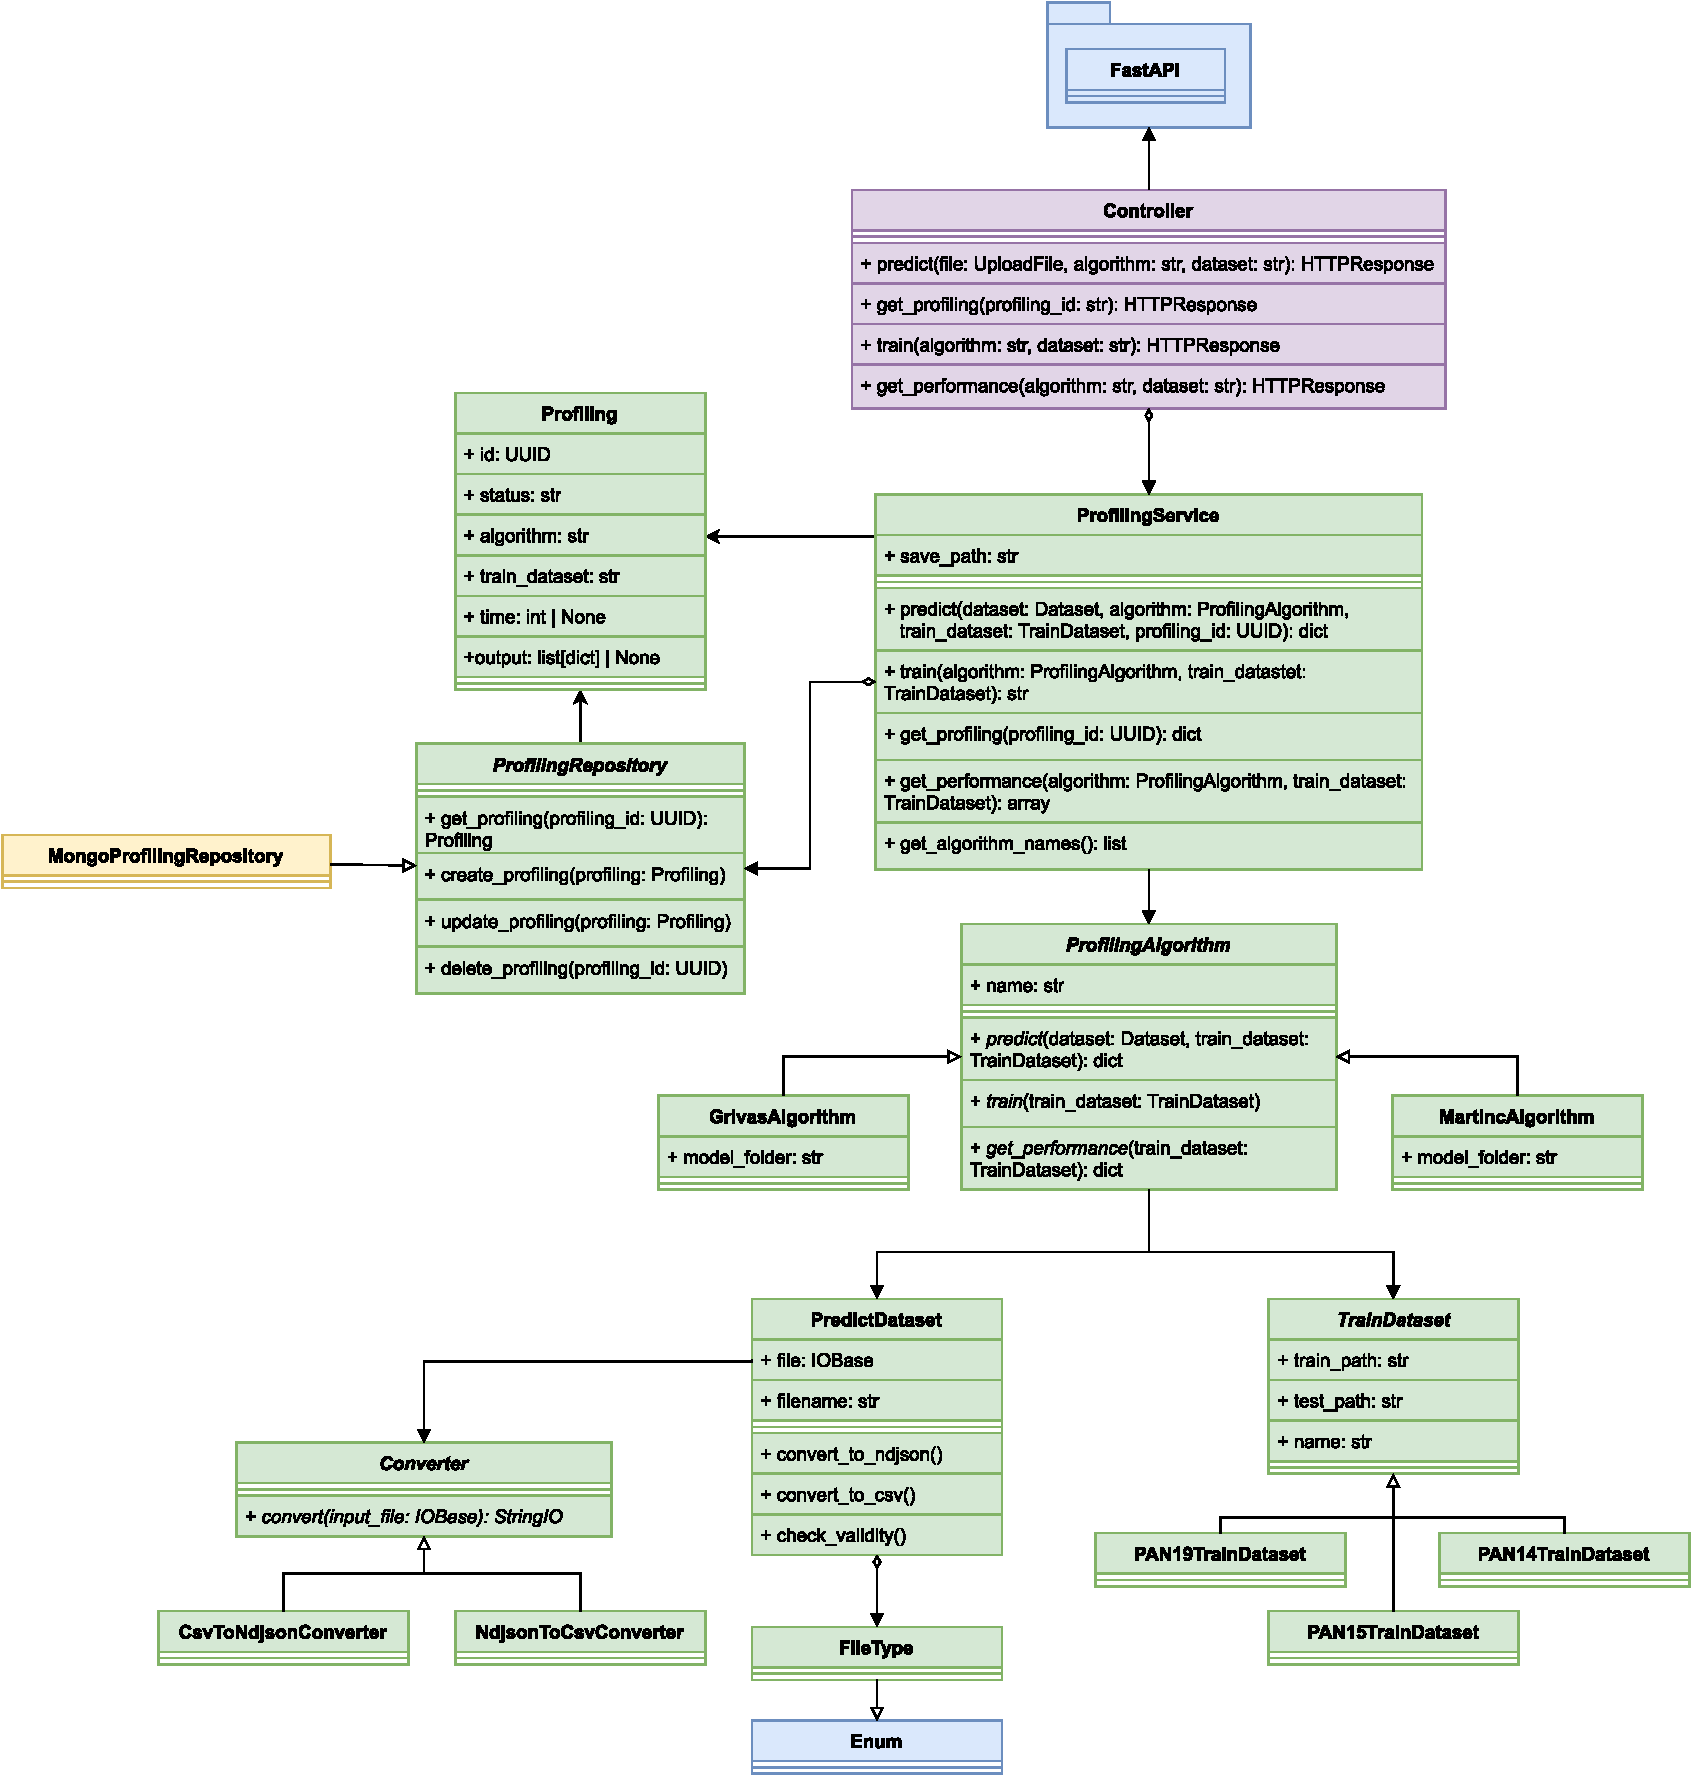
\includegraphics[width=\textwidth]{diagramas/clases_back.pdf}
	\caption{Diagrama de clases de la implementación del \textit{backend}}
	\label{fig:implementacion_clases_backend}
\end{figure}

\section{\textit{Frontend}}

En lo que respecta a la implementación del \textit{frontend}, como se explicó en la Sección \ref{sec:herramientas_frontend}, se optó
por utilizar NextJS como \textit{framework} de desarrollo, el cual está basado en React. Así, teniendo esto en cuenta y apoyándonos
en el diagrama de clases de la Figura \ref{fig:implementacion_clases_frontend}, analizaremos
las clases más relevantes del proyecto y su relación con el resto de módulos y componentes.

\bigskip
Primero, como elemento principal que conforma la interfaz de usuario, estarían todas las páginas que se encuentran en el módulo \textit{pages}, es decir,
la página principal o \textit{landing} (\textit{Home}) y la página de resultados (\textit{Results}).

\bigskip
Como se ve reflejado en el diagrama, cada página está formada por varios componentes, los cuales se almacenan dentro del módulo \textit{components}.
En este sentido, el componente \textit{Chart} es uno de los más complejos e interesantes, dado que en él reside toda la lógica y la configuración común
 de los gráficos que se muestran en el \textit{dashboard} de la página de resultados. Otros componentes importantes son el \textit{UploadDataset},
el cual se encarga de gestionar los eventos de \textit{drag and drop} y de la subida de archivos; el componente \textit{AlgorithmCard}, que
presenta la información de las caraterísiticas que perfila cada algoritmo y se ocupa de mostrar el \textit{tooltip} con la información detallada;
o el componente \textit{PeopleList}, el cual se hace cargo de manejar la paginación, la ordenación y la selección de la lista de personas.

\bigskip
Es importante
destacar aquí el hecho de que cada uno de los componentes tiene una hoja de estilos propia gracias a la utilización de los módulos CSS \cite{cssmodules}. A su vez
se buscó sacarle partido a SASS, haciendo uso de variables globales que definen colores o distancias; empleando el anidamiento para una mejor
estructuración de los estilos; y utilizando los \textit{mixins}, esto es, funciones que permiten reutilizar código CSS para, por ejemplo, simplificar la implementación de las \textit{media queries}. En este
sentido, para cumplir con el requisito no funcional de portabilidad explicado en la Sección \ref{sec:analisis_requisitos_no_funcionales}, 
era necesario que la aplicación fuese \textit{responsive}, es decir, adaptable a cualquier tamaño de pantalla, desde móviles a monitores.


\bigskip
Por otro lado, ya que algunos componentes y páginas necesitan realizar peticiones al \textit{backend}, es necesario implementar un servicio
que mantenga la lógica de la comunicación y exponga funciones que faciliten su uso. De esta tarea se encarga la clase abstracta \textit{ProfilingService},
la cual define funciones estáticas tales como \textit{getProfiling()} o \textit{predict()} que abstraen al resto de componentes de la lógica de las peticiones HTTP.
Dicho servicio hace uso por debajo de \textit{fetch}, una API nativa de JavaScript muy flexible que permite programar casi cualquier funcionalidad
relacionada con peticiones HTTP. Asimismo, ya que la asincronía es un concepto muy extendido y necesario en el desarrollo web, se ha optado
por usar las \textit{Promises} de JavaScript, las cuales permiten realizar operaciones asíncronas de forma muy sencilla.

\bigskip
Por último, como toda aplicación tipada, es necesario definir un modelo de datos que represente cada entidad. En este sentido, se ha optado
por el uso de enumeraciones o \textit{enums} para representar la mayor parte de los datos, tales como los algoritmos de perfilado, los géneros,
las edades o los rasgos personales. Asimismo, se ha creado una clase \textit{Person} que aúna todas las características
perfiladas de una persona junto a su nombre. Finalmente, para representar los datos enviados por el \textit{backend}, se ha definido la clase \textit{ProfilingDto},
la cual, en última instancia, permite realizar la conversión a la clase \textit{Profiling} empleada por el resto de la aplicación.


\bigskip
\begin{figure}[H]
	\centering
	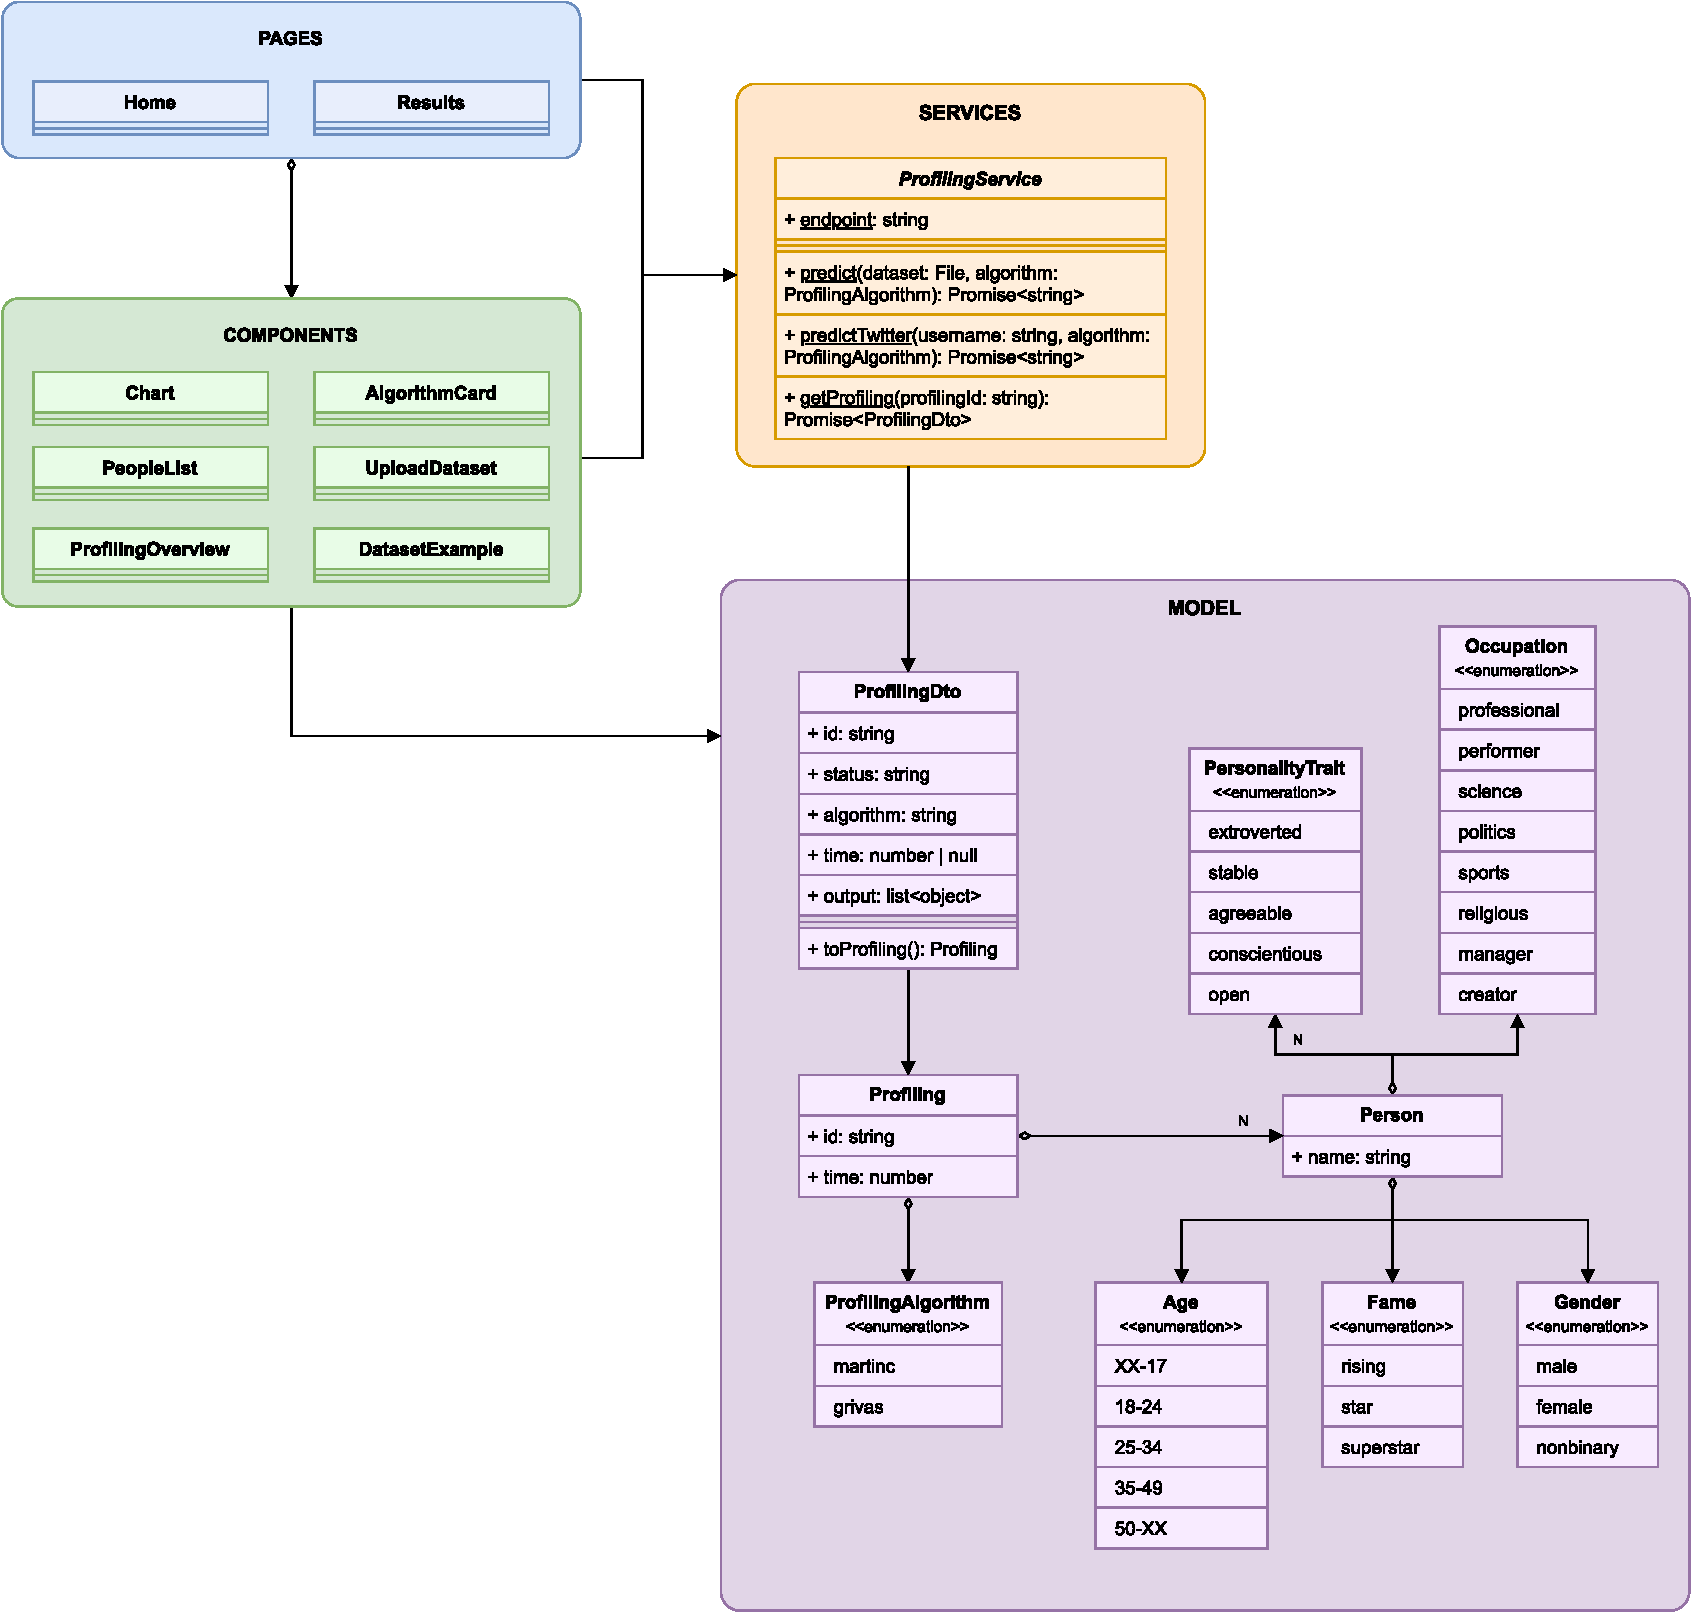
\includegraphics[width=\textwidth]{diagramas/clases_front.pdf}
	\caption{Diagrama de clases de la implementación del \textit{frontend}}
	\label{fig:implementacion_clases_frontend}
\end{figure}
